%%MaD.tex - Notes taken for Materials and Devices Lecture
%%Author: Andy Goetz
%%Date Modified: 10-7-09
%%License: Ask me before reproducing/modifying, etc.


\documentclass{article}

%Make sure you have the file ShumanNote.scy in the same directory as
%this one. It has contains the style sheet for ECE111, and is needed
%to standardize the layout of LateX documents created for the class.
%%Modified by Andy Goetz 10-13-09, changed font to Arev, look at font
%%section for details.

\NeedsTeXFormat{LaTeX2e}[1994/06/01]

%% load up the fancy box making package
\usepackage{fancybox}
\usepackage{graphicx}
\usepackage{float}
\usepackage[colorlinks=true,linkcolor=black, urlcolor=black,linkcolor=black]{hyperref}
\usepackage[letterpaper, portrait]{geometry}
%% Load up PS insertion package
\usepackage{psboxit}
\PScommands
\textheight = 9in
\footskip = 20pt

%This section was added by Andy Goetz on 10-13-09. It replaces the
%Arial font with the Arev font, which has math mode support so that
%math functions match the look and feel of the rest of the document
\usepackage[T1]{fontenc}
%\usepackage{arev}

%Commented out by Andy Goetz on 10-13-09, replace by different code
%for font selection
% \renewcommand{\rmdefault}{phv} % Arial
%\renewcommand{\sfdefault}{phv} % Arial
%% Load up fancy headers and footers package
\usepackage{fancyhdr}

%% now reset the headers and footers
\fancyhead{}
\fancyfoot{}
% Header/footer Thickness
\renewcommand{\headrulewidth}{1pt}
%\renewcommand{\footrulewidth}{0.4pt}

%Commented out by Andy Goetz on 10-13-09, as LateX was giving warnings
%about \warning being defined twice.

% Warning Box with 2 parameters. Param 1: Picture, Param2: Text
%\newcommand{\warning}[2]{\begin{table}[ht!tbp]
%\begin{center}
%\begin{tabular}{c c}
%
%#1 \hspace{5mm} & \framebox{\parbox[r]{4in}{#2}} \\ [3ex]
%\end{tabular}
%\end{center}
%\end{table}}

\newcommand{\doublespace}{\newline \newline}

% Side by Side Pictures Param1: Graphic insert, Param2: Caption for Graphic1, Param3:Label for Graphic1, Param4: Graphic insert, Param5:Caption for Graphic2, Param6:Graphic2 label
\newcommand{\picsidebyside}[6]{\begin{figure}[ht]            
\begin{minipage}[b]{0.5\linewidth}
\centering
#1
\caption{#2}
\label{#3}
\end{minipage}
\hspace{0.5cm}
\begin{minipage}[b]{0.5\linewidth}
\centering
#4 
\caption{#5}
\label{#6}
\end{minipage}
\end{figure}}

% Center Image Command
\newcommand{\centerimage}[3]{
\begin{figure}[htbp]  
\begin{center}
#1
\caption{#2}
\label{#3}
\end{center}
\end{figure}}


\setlength\fboxsep{3pt}
\setlength\fboxrule{0.5pt}

\newcommand{\centerlisting}[3]{
\centerimage{
\fbox{
#1
}
}{#2}{#3}
}


\newcommand{\createtitle}[2]{
%% bring the style into effect
\pagestyle{fancy}

\lfoot{ECE510}
\rfoot{\thepage}
\rhead{A. Goetz, P. Lamb, K. Riedl}
\lhead{#1}

\begin{titlepage}
 
\begin{center}
 
 
\textsc{\LARGE ECE 510 System Verilog}\\[1.5cm]
 
\textsc{\Large Portland State University}\\[0.5cm]
 
 
% Title
\HRule \\[0.4cm] { \huge \bfseries #1}\\[0.4cm]
 
\HRule \\[1.5cm]
 
% Author and supervisor
\begin{minipage}{0.4\textwidth}
\begin{center} \large
Andy \textsc{Goetz} \& Phil \textsc{Lamb} \& Kevin \textsc{Riedl}\\
\end{center}
\end{minipage}

\vspace{1cm}
%\includegraphics[height=4.75in]{sh_landing_gear.png}
 
 
\end{center}
\begin{center}#2\end{center}
\vfill
\begin{center}
% Bottom of the page
{\large \today}

\end{center} 
\end{titlepage}

\newpage
\thispagestyle{empty}
\vspace*{0.6\paperheight}
\begin{center}\textit{This page intentionally left blank.}\end{center}

\newpage
\setcounter{page}{1}



}

%%
%% End of file `phdthesis.sty`
 
\usepackage{algorithm}
\usepackage{algpseudocode}
\usepackage{tikz}
\usepackage{array}
\usepackage{program}
\usepackage{listings}
\pdfpagewidth 8.5in 
\pdfpageheight 11in
\usepackage{titlesec}
\usepackage{ucs}
\usepackage[utf8x]{inputenc}
%% \titleformat{\section}{\bfseries}{\thesection}{1em}{}
%% \titleformat{\subsection}{\bfseries}{\thesubsection}{1em}{}
%This package is used to line up pictures 
\usepackage{graphicx}
\usepackage{fancyvrb}
\usepackage{listings}
%allows cursive font
%\usepackage{amsmath}

%allows hyperlinks 
\usepackage{hyperref}

%use newlines instead of indentation between paragraphs
\usepackage[parfill]{parskip}

\newcommand{\HRule}{\rule{\linewidth}{0.5mm}} 
%% \renewcommand\thesubsection{\alph{subsection})}
%% \renewcommand\thesection{\arabic{section})}

\begin{document}

\createtitle{Gameboy Graphics Proposal}{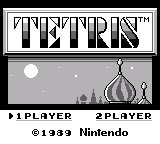
\includegraphics{tetris.png}}
%% These commands allow me to use cursive letter for things such as
%% length.  Note that on ubuntu linux, this required installation of
%% the package 'texlive-fonts-extra'. 
%% Taken from
%% http://www.latex-community.org/forum/viewtopic.php?f=5&t=1404&start=0
\newenvironment{frcseries}{\fontfamily{frc}\selectfont}{}
\newcommand{\textfrc}[1]{{\frcseries#1}}
\newcommand{\mathfrc}[1]{\text{\textfrc{#1}}}




\section{Overview}
We plan on implementing the sprite-based graphics of the original
gameboy. The gameboy used raster graphics accessed through a simple,
memory mapped interface. We plan on creating an implementation of these
graphics, and leveraging the new validation features of System Verilog
to accelerate the testing process. 

\section{Existing Work}
The internet is full of gameboy emulators. In addition, several
emulators have been created for FPGAs (i.e.
\url{https://github.com/trun/fpgaboy}). However, none of these designs
use System Verilog. We plan on using these designs as a jumping-off
point for our own implementation.

While there is no publicly released design documentation for the 
Gameboy there are a number of resources created by hobbyists who 
have reverse engineered the Gameboy hardware and software.

\section{Requirements}

We plan on implementing the original gameboy's sprite-based raster
graphics engine. In addition to accepting draw commands from the
gameboy cpu, the graphics engine needs to provide interrupt signals to
the CPU. 

The graphics module will be implemented and tested in isolation, 
but we plan to integrate our module with another group's Gameboy CPU 
implementation if time allows.  In addition, we plan to synthesize
the full design on an Altera Cyclone II if time allows.
For video output this may include writing a module to conver our 
video output to VGA.


\section{Testing Methodology}
The testing will be implemented with the transaction based
emulation mode on the Veloce hardware emulator. Since the 
actual Gameboy specifications are closed source, the test 
bench will verify the behavior of the graphics module as
described in the documentation from the Existing Work 
section.



\end{document}

